\section{Background}
\label{sec:background}

A generalized search tree is a balanced tree whose node occupies one page. Each
entry of an internal node is a pair (key, downlink), and the key covers the keys
of all entries in the referenced subtree. A search descends into every subtree
whose key may contain an answer, so unlike in a B-tree several descent paths may
be active simultaneously; the cost of a search is governed by how many they are.

An operator class supplies the data-specific operations. In PostgreSQL these are
\code{consistent} (may this subtree contain an answer?), \code{union} (a key
covering a set of keys), \code{penalty} (the cost of extending a key by an
entry), \code{picksplit} (partition an overflowing node in two), \code{same},
the optional \code{compress}, \code{decompress} and \code{fetch}, and the
optional \code{distance} for nearest-neighbour search. The first four determine
the shape of the tree completely: substituting bounding rectangles yields an
R-tree, substituting signatures yields a full-text index, substituting ranges
yields a range index.

Two properties of this interface matter throughout the paper. First, it contains
no ordering operation, and none of the operations induces one. Second,
\code{picksplit} encodes the operator class author's own notion of a good
partition. We will use exactly that notion in Section~\ref{sec:overlap} rather
than inventing a criterion of our own; this is what keeps the construction
algorithm framework-level rather than specific to a key type.

Concurrency follows Kornacker \cite{kornacker1997concurrency}: pages of a level
are chained by right links, and a split is arranged so that a search arriving at
a page that has been split can still reach the data by following the right link,
without holding a lock on the parent. A detailed account of the implementation
is given in \cite{rogov2026}.

\section{Related work}
\label{sec:related}

\paragraph{Sort-based packing of R-trees.} Roussopoulos and
Leifker~\cite{roussopoulos1985direct} build a packed R-tree by sorting
rectangles on a coordinate and filling nodes consecutively. Kamel and
Faloutsos~\cite{kamel1993hilbert} sort on the Hilbert value of the centre,
obtaining better locality. Leutenegger et al.~\cite{leutenegger1997str} propose
sort-tile-recursive packing, which partitions space into slabs; Garc\'ia et
al.~\cite{garcia1998greedy} choose the partition greedily; B\"ohm and
Kriegel~\cite{bohm1999bulk} address the high-dimensional case. Achakeev et
al.~\cite{achakeev2012sort} make the packing adaptive to an expected query
profile and later parallelise it~\cite{achakeev2013parallel}; recent work
learns the partitioning policy~\cite{qi2023platon}. All of this line is
formulated in terms of coordinates, of the area of a bounding rectangle, or of
a query profile over such objects. An operator class over signatures or over
ranges provides none of these, so none of the algorithms transfers to the
framework setting as stated.

\paragraph{Generic bulk loading.} The closest prior work is van den Bercken et
al.~\cite{bercken1997generic}, who give a bulk loading algorithm explicitly
called generic: it applies to a wide range of index structures, level by level,
using Arge's buffer tree to batch insertions. Arge et
al.~\cite{arge2002bulk} extend the approach from loading to bulk updates and
queries, and the Priority R-tree~\cite{arge2004priority} attains worst-case
optimal query bounds.

The distinction from the present work is worth stating precisely, because the
word ``generic'' is the same and the meaning is not. Buffer-tree loading is
generic over structures that have an insertion algorithm: it batches insertions
so that each of them is cheap in expectation, and it therefore requires no
order on keys, which is exactly why it is applicable so widely. What it
produces is the tree that insertion would have produced, at lower I/O cost:
pages are filled by splits, and the shape is the shape insertion gives. Sorted
packing requires more from the operator class---an order preserving
locality---and gives more in return: pages are filled to the configured factor
rather than by splitting, and the shape is determined by the order and by the
choice of split points rather than by the history of insertions. The two are
complementary, and neither dominates: buffer-tree loading is the method of
choice when no locality-preserving order exists, which for some operator
classes is the case.

Our contribution is therefore not bulk loading that is generic in the sense of
requiring nothing from the structure, but the identification of the minimal
thing a framework must \emph{require} for the sorted variant to be available at
all---and of what it must then do so that the result is not worse than what
insertion would have given.

\paragraph{Split quality.} The R*-tree~\cite{beckmann1990rstar} improves the
shape of the tree by accounting for perimeter and by forced reinsertion; the
RR*-tree~\cite{beckmann2009rrstar} refines subtree choice on insertion. These
optimise the tree built by insertion. An attempt to improve the penalty
function of a generalized search tree along the same lines
\cite{borodin2017penalty} proved inapplicable in a production system: changing
the penalty function changes the shape of indexes built by earlier versions, and
a database system must keep existing indexes usable after an upgrade. Sorted
construction is free of that constraint, because it affects only newly built
indexes---a point worth recording, since it explains why the same idea
succeeds in one form and fails in another.

\paragraph{Extensible index frameworks.} The generalized search
tree~\cite{hellerstein1995generalized} is the framework studied here;
concurrency and recovery for it are due to Kornacker et
al.~\cite{kornacker1997concurrency}. A parallel line covers space-partitioning
structures: SP-GiST and its realization in
PostgreSQL~\cite{eltabakh2006spgist} raise the same class of question---what
the framework must ask of the extension---for a different family of trees. The
extensible index machinery of PostgreSQL as it stands is documented
in~\cite{rogov2026}.

\paragraph{Surveys.} Gaede and G\"unther~\cite{gaede1998multidimensional} survey
multidimensional access methods; Graefe~\cite{graefe2011modern,graefe2024more}
surveys B-tree techniques, including bulk construction, in the one-dimensional
setting where an order is given rather than requested. Comer's earlier
survey~\cite{comer1979ubiquitous} and the original B-tree
paper~\cite{bayer1972organization} fix the terminology we use for the
one-dimensional case.

\paragraph{Page-level optimisation.} An orthogonal way to speed up
insertion-based construction is to make the individual page update cheaper
\cite{borodin2017memory}. Intra-page indexing~\cite{borodin2019intrapage}
attacks the CPU cost of scanning a node; Section~\ref{sec:eval} shows why that
cost matters. Both are complementary to this work.

\paragraph{External-memory sorting.} The cost of the sorting step is that of
external merge sort in the standard I/O model~\cite{aggarwal1988io}.

\section{Cost model}
\label{sec:cost}

Let $N$ be the number of entries, $B$ the page size, $M$ the memory available
for sorting, $f$ the node fan-out, $\varphi$ the page fill factor, $H$ the tree
height, and $c_r$, $c_s$ the cost of a random and of a sequential page access.

Construction by insertion descends to a leaf for every entry:

\begin{equation}
\label{eq:ins}
P_{\text{ins}} = N\left(H + \gamma\right) c_r ,
\end{equation}

where $\gamma$ is the average number of extra accesses caused by splits and by
updates of parent keys. Construction by sorting costs an external sort followed
by a single sequential pass writing the packed levels:

\begin{equation}
\label{eq:sort}
P_{\text{sort}} = \frac{2N}{B}\log_{M/B}\frac{N}{B}\, c_s
                + \frac{N}{f\varphi}\, c_s .
\end{equation}

Three sources of gain are visible: random accesses become sequential, splits
disappear, and $\varphi$ rises from the $\approx 0.7$ characteristic of
split-produced pages to the configured fill factor. The last also shrinks the
index, and hence the cost of every later full scan of it.

The comparison is incomplete, because it accounts only for construction. Define
the \emph{overlap} of level $l$ as the expected number of level-$l$ nodes whose
key matches a random point query,

\begin{equation}
\label{eq:omega}
\omega_l = \mathbb{E}\bigl|\{\,u \in U_l : \code{consistent}(\mathit{key}(u), Q)\,\}\bigr| ,
\end{equation}

so that the cost of a point query is $\sum_l \omega_l\, c_r$. A node is visited
only if its parent was, which invites the conclusion that overlap compounds down
the tree. It does not. Measurement (Section~\ref{sec:eval}) shows that $\omega_l$
reaches a value characteristic of the construction method within one or two
levels of the root and stays there, so that

\begin{equation}
\label{eq:steady}
P_{\text{point}} \approx \omega_\infty H c_r .
\end{equation}

The quality of construction thus enters the cost of a search as a constant
factor at every step of the descent, and the correct basis for comparing
construction methods is $P_{\text{build}} + n P_{\text{point}}$ for the expected
number $n$ of queries over the lifetime of the index~--- not $P_{\text{build}}$
alone, which is what such comparisons customarily report.

\section{Sorted construction at framework level}
\label{sec:build}

\subsection{The support function}

We extend the operator class with one optional support function returning a
comparator over keys. If it is present, the index is built by sorting all
entries with that comparator, filling leaf pages consecutively up to the fill
factor, forming an entry for the level above from \code{union} of each completed
page, and repeating level by level until a single page remains.

The order must be declared by the operator class and not passed as a parameter
of the index. In an early version of the implementation the comparator was
supplied as a relation option, which allowed any function of matching signature to be named~--- that
is, allowed a silently incorrect index to be built \cite{thread-fast-build}.
Moving the declaration into the operator class makes the order part of the
definition of the index type and allows it to be validated at index creation.

\subsection{Locality-preserving orders}

For a point type we use the Z-order, or Morton code \cite{morton1966,
orenstein1984zorder}: coordinates are reinterpreted as unsigned integers and
their bits interleaved. Points close in space receive close $Z$ values; the
converse does not hold, but for construction this affects the quality of the
tree, not its correctness.

Two implementation details are worth recording. The bit pattern of an IEEE 754
value read as an integer is order-preserving for non-negative values and
reversed for negative ones; for preserving locality this suffices, since the
discontinuity occurs only at zero. Not-a-number values are unordered, and their
placement in the order is not neutral: it must agree with the behaviour of
\code{union} and \code{consistent}, which requires an explicit convention.

That the order is a property of the operator class and nothing else is
demonstrated in Section~\ref{sec:eval} by supplying the Hilbert curve as a
drop-in alternative: an operator class differing from the built-in one in
exactly one support function out of ten, with no change to the tree, to logging
or to the concurrency protocol.

\subsection{Bottom-up packing and right links}

Constructing bottom-up, the contents of a page are known before it is written,
so \code{union} is applied once per page rather than incrementally.

There is no concurrency during construction: no search and no split can occur.
Formally the right links of Kornacker's protocol therefore need not be set. We
set them nevertheless. The completeness of the right-link chain at every level
is a structural invariant that index verification tools check; if a sorted build
left it unsatisfied, a verification tool would have to distinguish indexes by
the way they were built. We state this as a design rule: an optimisation must
not reduce the set of checkable properties of a structure.

\section{Non-leaf key overlap}
\label{sec:overlap}

% Рисунки P1. Данные в графиках — из bench/results/ за 2026-08-02.

% --- Рисунок 1: почему разбиение по заполнению страницы даёт перекрытие.
% Одни и те же точки, один и тот же порядок обхода; различается только то, где
% проведены границы страниц. Слева — по заполнению, справа — по picksplit.
\begin{figure}[t]
\centering
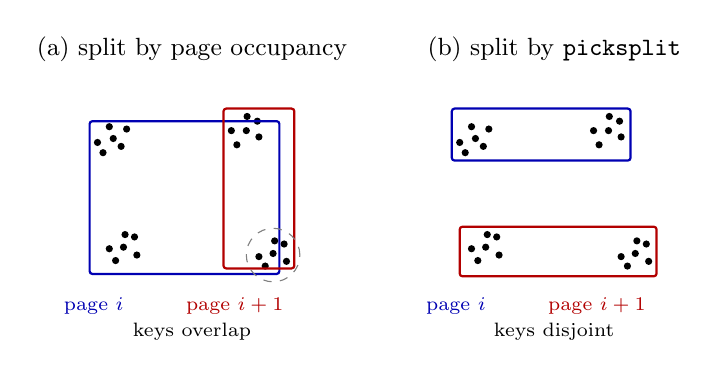
\begin{tikzpicture}[scale=1.0,
  pt/.style={circle, fill=black, inner sep=0pt, minimum size=2.6pt},
  key/.style={thick, rounded corners=1pt}]

% Четыре плотных скопления. Координаты заданы явно: на случайных точках
% эффект не читается.
% Четыре плотных скопления. Координаты заданы явно: на случайных точках
% эффект не читается.
\newcommand{\drawpoints}{%
  \foreach \p in {%
    (0.55,2.15),(0.70,2.35),(0.85,2.10),(0.62,2.02),(0.92,2.32),(0.75,2.20),
    (2.25,2.30),(2.45,2.48),(2.60,2.22),(2.32,2.12),(2.58,2.42),(2.44,2.30),
    (0.70,0.80),(0.90,0.98),(1.05,0.72),(0.78,0.65),(1.02,0.95),(0.88,0.82),
    (2.60,0.70),(2.80,0.90),(2.95,0.64),(2.68,0.58),(2.92,0.86),(2.78,0.74)}
    { \node[pt] at \p {}; }%
}

% ---------- (a) разбиение по заполнению страницы
\begin{scope}
  \node[anchor=south, font=\small] at (1.75,3.05) {(a) split by page occupancy};
  \drawpoints
  % порядок обхода ведёт по нижнему ряду, затем по верхнему; страница
  % заполняется до отказа, и граница приходится на середину скопления
  % порядок обхода приводит страницу к концу внутри правого нижнего скопления:
  % его точки достаются обеим страницам, и обе ограничивающие рамки тянутся
  % через всю занятую область
  \draw[key, blue!70!black] (0.45,0.48) rectangle (2.86,2.42);
  \draw[key, red!70!black]  (2.15,0.55) rectangle (3.05,2.58);
  \draw[dashed, gray] (2.78,0.72) circle (0.34);
  \node[font=\scriptsize, blue!70!black, anchor=north west] at (0.0,0.30) {page $i$};
  \node[font=\scriptsize, red!70!black, anchor=north west] at (1.55,0.30) {page $i+1$};
  \node[font=\scriptsize, anchor=north] at (1.75,-0.02) {keys overlap};
\end{scope}

% ---------- (b) разбиение функцией класса операторов
\begin{scope}[xshift=4.6cm]
  \node[anchor=south, font=\small] at (1.75,3.05) {(b) split by \texttt{picksplit}};
  \drawpoints
  \draw[key, blue!70!black] (0.45,1.92) rectangle (2.72,2.58);
  \draw[key, red!70!black]  (0.55,0.45) rectangle (3.05,1.08);
  \node[font=\scriptsize, blue!70!black, anchor=north west] at (0.0,0.30) {page $i$};
  \node[font=\scriptsize, red!70!black, anchor=north west] at (1.55,0.30) {page $i+1$};
  \node[font=\scriptsize, anchor=north] at (1.75,-0.02) {keys disjoint};
\end{scope}
\end{tikzpicture}
\caption{The same entries under the same order; only the choice of page
boundaries differs. Filling each page to capacity (a) puts the boundary in the
middle of a dense region, so the bounding keys of two neighbouring pages cover
almost the same area and a query matching either enters both subtrees.
Delegating the choice to the operator class (b) lets boundaries follow the data
and the keys come out disjoint. Rectangles are the keys stored in the parent.}
\label{fig:split}
\end{figure}

% --- Рисунок 2: перекрытие по уровням не накапливается.
\begin{figure}[t]
\centering
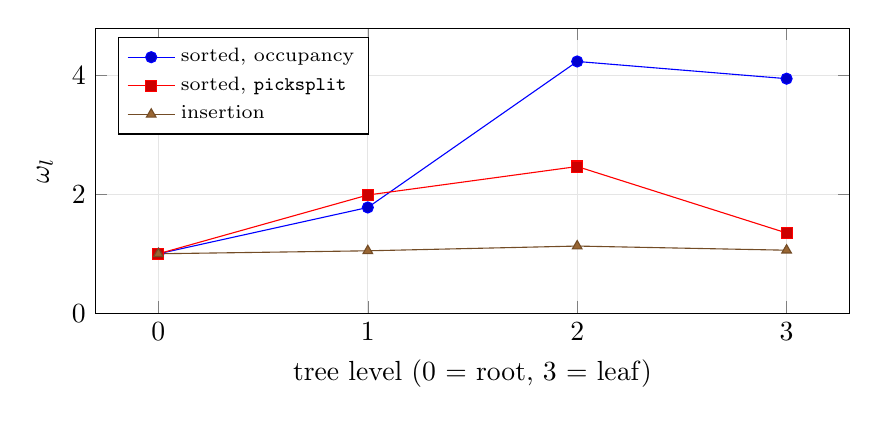
\begin{tikzpicture}
\begin{axis}[
  width=0.92\linewidth, height=5.2cm,
  xlabel={tree level (0 = root, 3 = leaf)},
  ylabel={$\omega_l$},
  xtick={0,1,2,3},
  ymin=0, ymax=4.8,
  legend pos=north west,
  legend style={font=\scriptsize, cells={anchor=west}},
  grid=major, grid style={gray!20},
  mark size=2pt,
]
\addplot+[mark=*] coordinates {(0,1.00) (1,1.78) (2,4.24) (3,3.95)};
\addlegendentry{sorted, occupancy}
\addplot+[mark=square*] coordinates {(0,1.00) (1,1.99) (2,2.47) (3,1.35)};
\addlegendentry{sorted, \texttt{picksplit}}
\addplot+[mark=triangle*] coordinates {(0,1.00) (1,1.05) (2,1.13) (3,1.06)};
\addlegendentry{insertion}
\end{axis}
\end{tikzpicture}
\caption{Overlap per level, $N = 10^7$ uniform points, 2000 probes. Each method
reaches a value characteristic of it within one or two levels of the root and
holds it; overlap does not compound with depth. The upper levels are bounded by
the number of nodes on them.}
\label{fig:levels}
\end{figure}

% --- Рисунок 3: зависимость от размера буфера.
\begin{figure}[t]
\centering
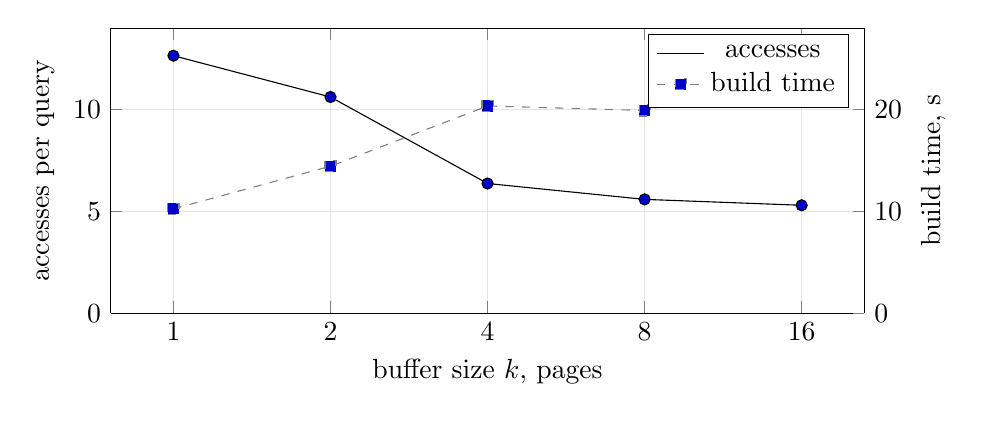
\begin{tikzpicture}
\begin{axis}[
  width=0.92\linewidth, height=5.2cm,
  xlabel={buffer size $k$, pages},
  ylabel={accesses per query},
  xmode=log, log basis x=2,
  xtick={1,2,4,8,16}, xticklabels={1,2,4,8,16},
  ymin=0, ymax=14,
  axis y line*=left,
  grid=major, grid style={gray!20},
  mark size=2pt,
]
\addplot+[mark=*, black] coordinates {(1,12.65) (2,10.62) (4,6.37) (8,5.59) (16,5.30)};
\label{plt:acc}
\end{axis}
\begin{axis}[
  width=0.92\linewidth, height=5.2cm,
  xmode=log, log basis x=2,
  xtick=\empty,
  ylabel={build time, s}, ylabel near ticks,
  ymin=0, ymax=28,
  axis y line*=right, axis x line=none,
  mark size=2pt,
]
\addlegendimage{/pgfplots/refstyle=plt:acc}\addlegendentry{accesses}
\addplot+[mark=square*, gray, dashed] coordinates {(1,10.25) (2,14.44) (4,20.36) (8,19.92) (16,23.58)};
\addlegendentry{build time}
\end{axis}
\end{tikzpicture}
\caption{Dependence on the buffer size, $N = 10^7$ uniform points. $k=1$
reproduces occupancy-based packing. The value shipped in PostgreSQL, $k=4$, is
conservative: $k=8$ improves query cost by 12\,\% at no cost in build time.}
\label{fig:bufsize}
\end{figure}


\subsection{Why occupancy-based packing fails}

Figure~\ref{fig:split} shows the mechanism. The procedure of
Section~\ref{sec:build} fills a page to the fill factor and
starts a new one, that is, chooses split points by a single criterion~---
occupancy. In one dimension that criterion is optimal. In more than one it is
not: an order preserves locality only approximately, and a page boundary falling
inside a dense region produces two neighbouring pages whose keys overlap
substantially.

The effect is large and it is not confined to the level at which it arises.
Measured per level on ten million uniform points, occupancy-based packing
settles at $\omega_\infty \approx 4$~--- a point query enters four subtrees at
every level instead of one.

\subsection{Delegating split selection to the operator class}

Rather than inventing a criterion for choosing split points, we use the one the
operator class already provides. Entries of a level are accumulated in a buffer
of $k$ pages; \code{picksplit} is applied to the buffer, recursively, until every
part fits on a page; the parts are written as pages of the level.

The buffer must be large enough that the partition algorithm can choose a cut
that does not coincide with a page boundary, and small enough that partitioning
stays cheap. Section~\ref{sec:eval} measures the dependence on $k$ and shows
that the value shipped in PostgreSQL, $k=4$, is conservative.

Note that this uses \code{picksplit} in a mode it was not designed for~---
partitioning a set larger than one page rather than an overflowing node~---
which is why the recursion is necessary, and which has a consequence that must
be stated: a split algorithm of super-linear complexity degrades when handed $k$
times as much data at once. For operator classes with such an algorithm we do
not enable sorted construction; improving their \code{picksplit} is a
prerequisite.

\section{Implementation}
\label{sec:impl}

The design is implemented in PostgreSQL and shipped in three releases: sorted
construction and the sort support interface of the operator class in release~14
(commit \code{16fa9b2b30a}), with validation of the support function
(\code{6f0bc5e1daf}) and right links set during construction
(\code{265ea567852}); split selection by \code{picksplit} over a buffer in
release~15 (\code{f1ea98a7975}); sorted construction for the
\code{btree\_gist} operator classes, made the default strategy, in release~18
(\code{e4309f73f69}). The discussions that led to the design, including
alternatives that were rejected, are publicly archived
\cite{thread-fast-build,thread-btree-gist-sort}.

Being part of the standard distribution, the implementation is available to
every user of the system without additional steps, and every measurement below
is reproducible on public releases.

\section{Evaluation}
\label{sec:eval}

\subsection{Setup}

All measurements were taken on a 16-core AMD EPYC machine with 31~GiB of RAM,
\code{shared\_buffers} set to 8~GB and \code{maintenance\_work\_mem} to 1~GB.
Configurations differ only by the change under study; where a change is a commit,
the baseline is its immediate parent, built from the same tree.

The primary metric is the \emph{number of index page accesses per query},
obtained from \code{EXPLAIN (ANALYZE, BUFFERS)}. It equals $\sum_l \omega_l$ of
Section~\ref{sec:cost}, it is independent of the storage device, and it is
reproducible on other hardware. Wall-clock times are reported for construction,
where they are meaningful, and are stated with the caveats they deserve.

Query windows are scaled so that the expected number of matching rows does not
depend on the size of the dataset: $d = 0.5/\sqrt{N}$ for uniform data. For real
data the window was calibrated by measurement (Section~\ref{sec:eval-real}); a
window chosen by absolute size gives a hundred matching rows in dense regions
and measures selectivity rather than tree quality.

\subsection{Reconstructing per-level overlap}

Internal keys cannot be read directly: the page inspection extension decodes
index tuples with the tuple descriptor of the index, whose attribute type is the
column type rather than the storage type of the operator class, so that for
\code{point\_ops} a \code{box} is printed as a \code{point} and one of its
corners is silently lost. We therefore reconstruct keys bottom-up: the key of a
leaf page is the bounding box of its entries, the key of an internal node is the
union of its children's keys, and the topology is taken from the downlink
pointers, which the decoding defect does not affect. For a sorted build the
stored key equals this union exactly, so the reconstruction is not an
approximation.

\subsection{Overlap does not compound with depth}

Table~\ref{tab:levels} and Figure~\ref{fig:levels} give $\omega_l$ per level
for ten million uniform points.

\begin{table}[t]
\centering
\caption{Overlap per level, $N = 10^7$, 2000 probes}
\label{tab:levels}
\begin{tabular}{lrrrrrr}
\toprule
& \multicolumn{2}{c}{insertion} & \multicolumn{2}{c}{occupancy} & \multicolumn{2}{c}{\code{picksplit}} \\
\cmidrule(lr){2-3}\cmidrule(lr){4-5}\cmidrule(lr){6-7}
Level & nodes & $\omega_l$ & nodes & $\omega_l$ & nodes & $\omega_l$ \\
\midrule
0 (root) & 1 & 1.00 & 1 & 1.00 & 1 & 1.00 \\
1 & 8 & 1.05 & 3 & 1.78 & 5 & 1.99 \\
2 & 823 & 1.13 & 363 & 4.24 & 601 & 2.47 \\
3 (leaf) & 90\,076 & 1.06 & 60\,241 & 3.95 & 80\,737 & 1.35 \\
\bottomrule
\end{tabular}
\end{table}

Each method converges to a value characteristic of it within one or two levels
of the root and holds it: $\omega_\infty \approx 4.0$ for occupancy-based
packing, $\approx 1.3$ for \code{picksplit}-based partitioning, $\approx 1.05$
for insertion. The upper levels are an exception only because $\omega_l$ there
is bounded by the number of nodes. This is the empirical content of
\eqref{eq:steady}, and it explains why the ratio between methods stays constant
as the tree grows deeper.

\subsection{Uniform data}
\label{sec:eval-uniform}

\begin{table}[t]
\centering
\caption{Construction method, uniform data}
\label{tab:uniform}
\begin{tabular}{llrrr}
\toprule
$N$ & construction & build, s & pages & accesses/query \\
\midrule
$10^6$ & insertion & 4.38 & 9\,115 & 3.95 \\
$10^6$ & sorted, occupancy & 0.64 & 6\,063 & 10.01 \\
$10^6$ & sorted, \code{picksplit} & 1.48 & 8\,165 & 4.62 \\
\midrule
$10^7$ & insertion & 69.61 & 90\,908 & 5.19 \\
$10^7$ & sorted, occupancy & 8.65 & 60\,608 & 12.23 \\
$10^7$ & sorted, \code{picksplit} & 19.80 & 81\,277 & 6.10 \\
\bottomrule
\end{tabular}
\end{table}

Relative to insertion, occupancy-based packing builds 6.8 and 7.1 times faster
and makes queries 2.53 and 2.36 times more expensive.
\code{picksplit}-based partitioning builds 3.0 and 3.8 times faster and stays
within 17 and 18\,\% of insertion on query cost: it removes 89 and 87\,\% of the
penalty. The residual is the price of choosing split points within a buffer
rather than globally over a level.

Both sorted variants produce a \emph{smaller} index than insertion~--- by 33 and
11\,\% respectively~--- because splits leave pages about 70\,\% full while
consecutive packing fills them to the configured factor. The common expectation
that better tree quality costs space does not hold here.

Table~\ref{tab:clustering} varies the degree of clustering: entries are drawn
from $N/(cf)$ dense clusters of $cf$ points each, where $f$ is the measured leaf
fan-out, so that $c$ is the size of a cluster in units of page capacity.

\begin{table}[t]
\centering
\caption{Accesses per query by cluster size, $N = 10^6$}
\label{tab:clustering}
\begin{tabular}{lrrr}
\toprule
$c$ & occupancy & \code{picksplit} & ratio \\
\midrule
uniform & 9.92 & 4.69 & 2.12 \\
0.5 & 9.65 & 3.48 & 2.77 \\
1 & 8.19 & 3.22 & 2.54 \\
2 & 7.78 & 2.88 & 2.70 \\
4 & 6.33 & 2.97 & 2.13 \\
8 & 6.36 & 2.52 & 2.52 \\
\bottomrule
\end{tabular}
\end{table}

The ratio stays in the range 2.1--2.8 throughout. We had expected a resonance:
the penalty should be largest when a cluster does not fit a whole number of
pages, so that boundaries systematically fall inside clusters, and smallest when
$c$ is integral. No such dependence appears. Clustered data does punish
occupancy-based packing somewhat harder than uniform data (2.5--2.8 against
2.12), which is consistent with the mechanism of Figure~\ref{fig:split}, but the
effect is not a function of $c$ in the way the mechanism suggests. Both build
time and index size are independent of $c$ to within one per cent.

\subsection{Is it the split rule, or merely the page count?}
\label{sec:eval-control}

In every measurement above, query cost falls as the number of index pages rises,
which admits a rival explanation: perhaps the benefit comes not from where the
split points are placed but from the tree being less bushy, with fewer entries
per page to examine. The classical estimate for a search tree in which all
children of a visited node must be examined puts the optimal branching factor at
about $e$, which makes the rival explanation plausible a~priori. It also has a
cheap remedy that would make this paper unnecessary: lower the fill factor.

Table~\ref{tab:control} tests it. Data and probes are generated from a fixed
seed, so both builds see the same ten million points and the same two thousand
queries.

\begin{table}[t]
\centering
\caption{Occupancy packing at reduced fill factor against \code{picksplit}, $N=10^7$}
\label{tab:control}
\begin{tabular}{llrr}
\toprule
Split rule & fill factor & pages & accesses/query \\
\midrule
\code{picksplit} & default & 81\,326 & \textbf{6.86} \\
occupancy & default & 60\,608 & 12.67 \\
occupancy & 80 & 68\,496 & 13.15 \\
occupancy & 70 & 78\,127 & 13.95 \\
occupancy & \textbf{65} & \textbf{84\,036} & \textbf{13.64} \\
occupancy & 60 & 91\,746 & 13.72 \\
occupancy & 50 & 109\,892 & 14.49 \\
\bottomrule
\end{tabular}
\end{table}

At an essentially equal page count---84\,036 against 81\,326---occupancy packing
costs 13.64 accesses per query against 6.86, twice as many. Lowering the fill
factor does not help at all; it mildly hurts, the cost drifting from 12.67 to
14.49 as the index grows by 80\,\%. The rival explanation is refuted: what the
operator class contributes is the placement of the boundaries, not the number of
them.

Two further remarks. First, the branching-factor argument holds only under
unbounded memory: a page is the unit of exchange with the buffer cache, and a
less bushy tree occupies more pages, fits it worse, and loses on data that does
not fit in memory---which on the real dataset of Section~\ref{sec:eval-real} is
the operating regime. Second, \code{picksplit}-based construction produced
81\,326 pages at both the default fill factor and at~65, that is, it does not
honour the parameter; we return to this in Section~\ref{sec:deployment}.

\subsection{Order and split points are separate levers}

Table~\ref{tab:factorial} crosses the two.

\begin{table}[t]
\centering
\caption{Accesses per query: order $\times$ split rule}
\label{tab:factorial}
\begin{tabular}{lrrrr}
\toprule
& \multicolumn{2}{c}{$10^6$ uniform} & \multicolumn{2}{c}{$1.38\times10^8$ OSM} \\
\cmidrule(lr){2-3}\cmidrule(lr){4-5}
Split rule & Z-order & Hilbert & Z-order & Hilbert \\
\midrule
occupancy & 10.01 & 5.57 & 15.30 & 10.17 \\
\code{picksplit} & 4.62 & 4.11 & 8.30 & 8.27 \\
\bottomrule
\end{tabular}
\end{table}

On uniform data the two are partially interchangeable: the curve recovers
44\,\% of the penalty of occupancy-based packing, the split rule recovers
53\,\%, and together they come within 4\,\% of insertion. On real data the
relation is asymmetric: the curve recovers 33\,\% while split points are chosen
by occupancy, and nothing at all once they are chosen by the operator class.
An elaborate space-filling order therefore pays off only while the partitioning
rule stays naive~--- a conclusion that matters to whoever writes an operator
class, and one that would have been invisible on synthetic data alone.

Build times for the Hilbert variant are not comparable with Z-order: the
experimental comparator used here does not implement abbreviated keys, so the difference
measures the presence of a sorting optimisation rather than a property of the
curve.

\subsection{Buffer size}
\label{sec:eval-buffer}

Table~\ref{tab:bufsize} and Figure~\ref{fig:bufsize} give the dependence.

\begin{table}[t]
\centering
\caption{Dependence on buffer size $k$, $N = 10^7$ uniform}
\label{tab:bufsize}
\begin{tabular}{rrrr}
\toprule
$k$ & build, s & pages & accesses/query \\
\midrule
1 & 8.89 & 54\,351 & 12.65 \\
2 & 13.05 & 81\,593 & 10.62 \\
4 & 15.71 & 81\,287 & 6.37 \\
8 & 19.99 & 81\,682 & 5.59 \\
16 & 23.35 & 81\,650 & 5.30 \\
\bottomrule
\end{tabular}
\end{table}

$k=1$ reproduces occupancy-based packing, as it must: there is nothing to choose
within a single page. The parameter is thus continuous between the two
strategies rather than a switch between them. The value shipped in PostgreSQL,
$k=4$, sits close to the knee: $k=8$ improves query cost by 12\,\% for 27\,\%
more build time, and $k=16$ by 17\,\% for 49\,\% more. Every step is a trade
rather than a free improvement, which is visible only in medians of repeated
runs: single build times at this scale vary by tens of percent
(Section~\ref{sec:threats}). Index size is independent of $k$ from $k=2$ on. Returns diminish sharply after $k=4$,
which is consistent
with the role of the buffer: it exists so that a cut need not coincide with a
page boundary, and by $k=8$ there is enough freedom for that.

\subsection{Real data}
\label{sec:eval-real}

We use 138\,078\,566 node coordinates from the OpenStreetMap extract of the
Netherlands. The index occupies 6.5--8.8~GB against 8~GB of buffer cache, so
unlike every preceding measurement it does not fit in memory.

Node density varies by orders of magnitude, and probes drawn from the data land
in cities. Calibration: a window of $5\times10^{-5}$ degrees returns 2.7 rows on
average, one of $5\times10^{-4}$ returns 112. We report both~--- the first as a
point query, the second as a deliberately non-selective one.

\begin{table}[t]
\centering
\caption{OSM, $N = 1.38\times10^8$; 5000 selective and 500 non-selective probes}
\label{tab:osm}
\begin{tabular}{lrrrr}
\toprule
construction & build, s & pages & selective & non-selective \\
\midrule
insertion & 1\,160.3 & 1\,285\,510 & 16.73 & 40.95 \\
sorted, occupancy & 322.7 & 836\,842 & 15.30 & 61.01 \\
sorted, \code{picksplit} & 396.3 & 1\,128\,374 & 8.30 & 48.23 \\
\bottomrule
\end{tabular}
\end{table}

Three observations.

The ratio between the two sorted variants, 1.84, agrees with the 2.0--2.2
measured on uniform data: the central result transfers to real data unchanged.

On non-selective queries the ratio falls to 1.26. When a query returns hundreds
of rows its cost is dominated by reading them rather than by navigation. This is
a boundary of applicability worth stating plainly: the construction method
matters for selective queries and is nearly irrelevant for scanning large
regions.

The cost of good partitioning falls with scale but does not vanish:
\code{picksplit} costs 87\,\% more than occupancy-based packing at $10^7$ and
23\,\% more at $1.38\times10^8$, as I/O takes over an increasing share of build
time.

\subsection{An unexpected result}
\label{sec:eval-surprise}

On this dataset \emph{insertion is no better than occupancy-based packing}:
16.73 accesses per selective query against 15.30, while taking three times as
long to build as \code{picksplit} and producing the largest index. Against
\code{picksplit}, at 8.30, it is twice as expensive. On uniform data the
ordering was the opposite, with insertion nearly optimal
(Table~\ref{tab:levels}).

The margin over occupancy-based packing is 9\,\%, and we are deliberately
exact about how little that carries. It is close to the threshold below which we
treat differences as not established, and it is sensitive to the choice of
probes: measured against independently drawn probe sets rather than the single
fixed set used here, the same comparison ranges over a factor of two
(Section~\ref{sec:threats}). What survives is not a magnitude but a reversal~---
on skewed data the method with global information is at least as good as local
insertion, whereas on uniform data insertion wins comfortably.

The plausible explanation is that on strongly skewed data the decisions taken
during insertion~--- subtree choice and node split~--- are local, and their
errors accumulate; this is the classical weakness of the R-tree that the
R*-tree was designed to address \cite{beckmann1990rstar}. Sorted construction
has global information and is free of it. On uniform data there is nothing to
accumulate, which is why the effect does not appear there.

We report this as an observation requiring confirmation rather than as a
result: it rests on a single dataset, and its magnitude already shrank once
under a more careful measurement. If it holds, it changes
the standing of sorted construction from a trade of quality for speed into an
improvement on both axes for skewed data~--- that is, for the practically
interesting case.

\subsection{Where the CPU goes}

Table~\ref{tab:cpu} profiles a backend performing a spatial join of 200\,000
outer rows against the index, some two million result rows, with index and table
resident in the buffer cache so that no I/O is involved.

\begin{table}[t]
\centering
\caption{Backend CPU during descent, self time}
\label{tab:cpu}
\begin{tabular}{rll}
\toprule
Share & Function & What it is \\
\midrule
22.4\,\% & \code{gistScanPage} & loop over entries of a page \\
14.1\,\% & \code{gist\_point\_consistent} & the predicate itself \\
12.8\,\% & \code{hash\_search} & buffer lookup table \\
10.2\,\% & \code{heap\_page\_prune\_opt} & table side \\
6.7\,\% & \code{MemoryContextReset} & \\
5.7\,\% & \code{PinBuffer} & pinning pages \\
5.4\,\% & \code{heap\_hot\_search\_buffer} & table side \\
4.7\,\% & \code{FunctionCall5Coll} & invoking the predicate \\
3.3\,\% & \code{gistcheckpage} & \\
2.3\,\% & \code{gistdentryinit} & preparing an entry \\
\bottomrule
\end{tabular}
\end{table}

Work on entries of an index page accounts for 46.8\,\% in total, buffer handling
for 18.4\,\% and the table side for 15.6\,\%.

Two consequences. First, the mechanics of iterating over entries cost 1.6 times
more than evaluating the predicate, so the promising direction for CPU work is
to examine fewer entries rather than to make each examination cheaper. Second,
buffer lookup and pinning together account for 18.4\,\% and are proportional to
the number of pages visited, that is to $\omega_\infty$: the contribution of
this paper, argued so far in terms of I/O, yields a comparable saving in CPU on
data that fits in memory.

\section{Deployment experience}
\label{sec:deployment}

The design has shipped since release~14 (2021) and has been the default strategy
for the \code{btree\_gist} operator classes since release~18 (2025). Over that
period one substantive failure occurred, and it is instructive.

The first attempt to extend sorted construction to \code{btree\_gist} was
reverted on the day it was committed. Two defects were involved: one in the
regression test environment, and one substantive~--- the comparator for the
bit-string type used a comparison that does not agree with the semantics of the
type. Work resumed four years later with an implementation written from scratch
\cite{thread-btree-gist-sort}.

The lesson is about framework design rather than about that patch. Consistency
of the comparator with \code{union} and \code{consistent} is a property of the
operator class that cannot be established by testing the build: an inconsistent
comparator yields an index that looks well-formed and silently loses part of the
answers. It is checkable only as a structural invariant of the produced tree,
namely that every parent key covers the keys of its children. A framework that
introduces a new support function is thereby obliged to introduce the check of
the corresponding invariant as well; we did not do so at the time, and the
omission cost four years.

\section{Threats to validity}
\label{sec:threats}

\paragraph{Reconstruction of internal keys.} Per-level overlap rests on keys
recovered bottom-up rather than read from the page. The recovery is exact for a
sorted build, where the stored key equals the union of the children's keys by
construction, and it is exact for the insertion-built index only if no key has
been left wider than that union. Deletions can leave such keys behind; our
datasets are insert-only, so the concern does not arise here, but a measurement
over a workload with deletions would need the keys read directly. That in turn
requires fixing the decoding of internal keys in the page inspection extension,
which currently interprets them with the tuple descriptor of the index rather
than the storage type of the operator class and silently drops part of a key
whenever the two differ.

\paragraph{Counters and times are not equally trustworthy.} The two must be
reported separately, and conflating them is easy. Accesses
per query, measured with both the data and the probe set fixed by seed, are
deterministic: they repeat to within a fraction of a percent, and every
page-access figure in Sections~\ref{sec:eval-uniform}--\ref{sec:eval-buffer}
carries that guarantee. Build times do not. Repeating the $10^7$ configurations
three times gave 6.78, 8.46 and 8.63~seconds for one and the same
configuration~--- a spread of 27\,\%. All times reported here are medians of
three sequential runs; we treat time differences below roughly 30\,\% as not
established, and ratios of times only when they exceed that.

\paragraph{Access counts depend on the choice of probes, and more so than times
depend on the machine.} On skewed data this is the larger threat of the two, and
it is not visible from a single run because the counter is perfectly repeatable
for a given probe set. One configuration on the OSM data gave 23.66 and 16.83
accesses per query for two independently drawn sets of 5000 probes. All real-data
figures reported here use one fixed set of 20\,000 probes, generated once and
shared by every index compared. Fixing the data by seed is not enough~--- the
queries must be fixed too, and on skewed data this matters more than anything
about the machine.

\paragraph{Window calibration on skewed data.} An early version of the real-data
experiment fixed the query window by absolute size. Because node density in
OpenStreetMap varies by orders of magnitude and probes are drawn from the data,
the window returned 112 rows on average instead of the intended one, and the
difference between construction methods shrank from a factor of two to 23\,\%.
The reported measurements calibrate the window by the expected number of
matching rows. Any comparison of index quality on skewed data is worthless
without this calibration, which is easy to overlook.

\paragraph{One operator class.} All quantitative results concern points, under
either of two orders. The claim that the technique is framework-level rests on
the interface argument and on the fact that a second order was added without
touching the framework, not on measurements over several key types. Operator
classes over signatures or ranges may behave differently, and we do not know
whether they do.

\paragraph{Comparison of curves by build time.} Invalid as measured: the
experimental Hilbert comparator does not implement abbreviated keys while the
built-in Z-order comparator does. Only the query-side comparison of curves is
sound.

\section{Limitations}

The method requires a locality-preserving order, and for operator classes whose
keys admit none it is inapplicable~--- with no diagnostic short of measuring
query quality. It requires a split algorithm that does not degrade on $k$ pages
of input. Its correctness rests on the consistency of the comparator with the
rest of the operator class, which the framework does not enforce. The gain does
not extend to subsequent maintenance: entries inserted after the build follow the
ordinary insertion path.

The measurements are confined to one operator class for points and its Hilbert
variant, to two synthetic distributions and one real dataset, and to a single
run per configuration. The comparison of curves by build time is invalid until
abbreviated keys are implemented for the Hilbert comparator. The result of
Section~\ref{sec:eval-surprise} requires confirmation.

\section{Conclusion}

Bulk loading of an extensible index framework reduces to sorting given one
additional support function, and the order it declares must come from the
operator class because nothing else knows it. The reduction alone is not a usable
result: choosing page boundaries by occupancy raises the steady-state overlap
from about 1.3 to about 4, and the index is built several times faster and
answers selective queries twice as expensively. Delegating the choice of split
points back to the operator class, over a buffer of several pages, removes
87--89\,\% of that penalty. Both parts are implemented in PostgreSQL and shipped
to its users.

The order and the split rule are separate levers with an asymmetric interaction:
on real data an elaborate curve helps only while the split rule is naive. The
buffer size shipped in the implementation is conservative by 12\,\%. And the
question of whether sorted construction is merely faster than insertion, or
actually better on skewed data, is open and worth settling.
